\section{Atividades}

Calcular a resistência equivatente total dos circuitos.

\subsection{ Circuito 1}
\begin{figure}[H]
  \centering
  \label{fig:ativ1}
  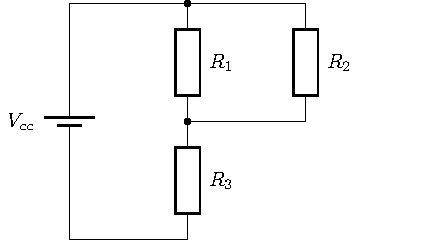
\includegraphics[scale=1.0]{fig-ativ1}
\end{figure}

\subsection{ Circuito 2}
\begin{figure}[H]
  \centering
  \label{fig:ativ1}
  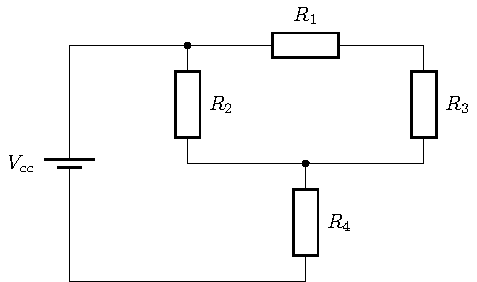
\includegraphics[scale=1.0]{fig-ativ2}
\end{figure}

\subsection{ Circuito 3}
\begin{figure}[H]
  \centering
  \label{fig:ativ1}
  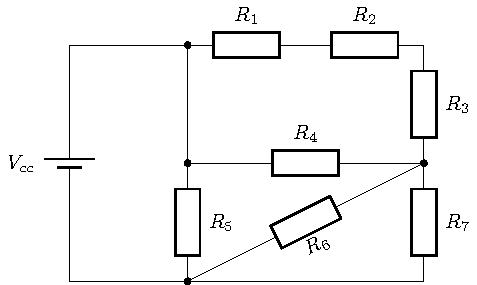
\includegraphics[scale=1.0]{fig-ativ3}
\end{figure}
